\chapter{LITERATURE SURVEY}
\label{chap:lit}

This section discusses various state-of-the-art algorithms that have been developed. Ideas from these algorithms have been used in implementation of the parallel algorithm.

\section{Generic Algorithm}

The Generic Algorithm is template that is used most of the algorithms discussed in upcoming sections. Most of the popular algorithms are variations of the generic algorithm. It must be noted that the efficiency of algorithms depends on the heuristics used for pruning the candidate list and selecting the order of vertices that are to be matched. The Generic Algorithm uses backtracking for finding the solutions. If we find out that solution cannot be achieved from a call, we end that call and proceed to the next.

\begin{algorithm}

\caption{\textsc{GenericAlgo}}\label{euclid}

\begin{algorithmic}[1]

%\textbf{Input:} Data graph g, Query graph q.\\

%\textbf{Output:} all subgraph isomorphisms of q in g.

\State $M \gets \emptyset$

\ForAll{$u \in V(q)$}

\State $C(u) \gets \textsc{FilterCandidates}$

\If{$c = \emptyset$}

\State \textbf{return}

\EndIf

\EndFor

\State $\textsc{SubgraphSearch}$ 

\Procedure{$\textsc{SubgraphSearch}$}{}

\If{$|M| = |V(q)|$}

    \State \textbf{report} M

    \Else

    \State $u \gets \textsc{NextQueryVertex}(..)$

    \State $C_R \gets \textsc{RefineCandidates}(...)$

    \ForAll{$V \in C_R$ such that v is not yet matched}

        \If{\textsc{IsJoinable}}

            \State \textsc{UpdateState}

        \EndIf

    \EndFor

\EndIf

\EndProcedure

\end{algorithmic}

\end{algorithm}

Algorithm 1 shows a generic subgraph isomorphism algorithm, \textsc{GenericAlgo}. Its inputs are a query graph q and a data graph g, and its output is a set of subgraph isomorphisms (or embeddings) of q in g. Here, to represent an embedding, we use a list M of pairs of a query vertex and a corresponding data vertex. The specific implementations of these procedures have been discussed in the respective subsections.

\section{Ullmann Algorithm}

Ulmann Algorithm was proposed in \cite{ullmann}. It exploits the template mentioned in Generic algorithm in the following way.\\
\\
\textsc{FilterCandidates:} \textsc{FilterCandidates} returns a set that contains the vertices whose label set is a subset of label set of $u$. For example, in figure $1$, it will return candidates of $u_1$ as \{$v_1, v_{1006}$\}\\
\\
\textsc{NextQueryVertex:} Returns the next data vertex that is to be checked. Ullmann Algorithm takes the vertices the the same order in which they appear in the input. Hence the result of this Algorithm highly depends on the input order. This issue is discussed in the next subsection.\\
\\
\textsc{RefineCandidates:} Prunes out all candidate vertices that have a smaller degree than u. In our running example, $v_{1005}$ will be pruned out as a candidate for $u_3$ because it has degree less than that of $u_3$ and hence can never map to it.\\
\\
\textsc{IsJoinable:} For all the vertices that have been matched, the \textsc{IsJoinable} checks whether there is a data edge corresponding to an edge in the query graph. In our running example, \{$u_1, u_2, u_3$\} will be matched to \{$v_1, v_2, v_3$\}. The \textsc{IsJoinable} procedure will check if there are corresponding edges between these matches. Since the edge between $v_2$ and $v_4$ is absent, the \textsc{IsJoinable} procedure will return false.

\section{VF2 algorithm}

This algorithm was published by \cite{vf2}. Following is the implementation of the algorithm in brief.

\textsc{NextQueryVertex:} VF2 Algorithm does not process data vertices in the order of input. Rather, from the start vertex, it returns the vertex which is a neighbour to the vertex (DFS like fashion). However, it does not use any particular method for selecting a neighbour. Hence, It does not exploit any property of the data/query graph.\\
\\
\textsc{RefineCandidates:} VF2 uses the following pruning
rules to prune out data vertex candidates:
\begin{enumerate}
    \item If there is vertex $v$ in the candidate list of a vertex $u$ that is not  connected to an already matched vertex, it is pruned out of the candidate list.
    \item If there is vertex $v$ in the candidate list of a vertex $u$, then the number of unmatched vertices connected to $v$ must be larger than those of $u$.
\end{enumerate}

\section{QuickSI Algorithm}

This algorithm was proposed in \cite{quicksi}.\\
\textsc{NextQueryVertex:} The QuickSI Algorithm exploits properties of the data and query graphs in order to prune candidate list more quickly and get better matching sequence compared to the previously discussed ones. It preprocesses the data graphs for increased efficiency by maintaining 'score' for each vertex. Scores are calculated by assigning weights to each vertex in accordance to frequency of its label and degree of the vertex. Then the algorithm selects the vertices in the order in which they appear in the minimum spanning tree. This heuristic is very efficient as the low label frequency vertices have lower probability of getting a candidate and hence will get pruned earlier. In most of the cases, QuickSI gives a better result than Ullmann and VF2 algorithm when run sequentially.


\section{Turbo\_iso Algorithm}

\begin{algorithm}
\caption{\textsc{$Turbo_{ISO}(g,q)$}}\label{euclid}
\begin{algorithmic}[1]
%\textbf{Input:} Data graph g, Query graph q.\\
%\textbf{Output:} all subgraph isomorphisms of q in g.
\State $u_s \gets \textsc{ChooseStartQueryVertex(q,g)}$
\State $q' \gets \textsc{ReWriteToNECTree}(q,u_s)$ // q': NEC Tree
\ForAll{$v_s$ in {$v|(v \in V(g))$ and $(L(u_s) \subseteq L(v))$}}
    \If{$\textsc{ExploreCR}(u'_s,{v_s},CR)=FAIL$}
        \State \textbf{continue}
    \EndIf
    \State order = $\textsc{DetermineMatchingOrder}(q',CR)$
    \State $\textsc{UpdateState}(M,F,{us},{vs})$
    \State $\textsc{SubGraphSearch}(g,q',q,order)$
    \State $\textsc{RestoreState}(M,F,{u_s},{v_s})$
\EndFor
\end{algorithmic}
\end{algorithm}

\begin{figure}[H]
\centering 
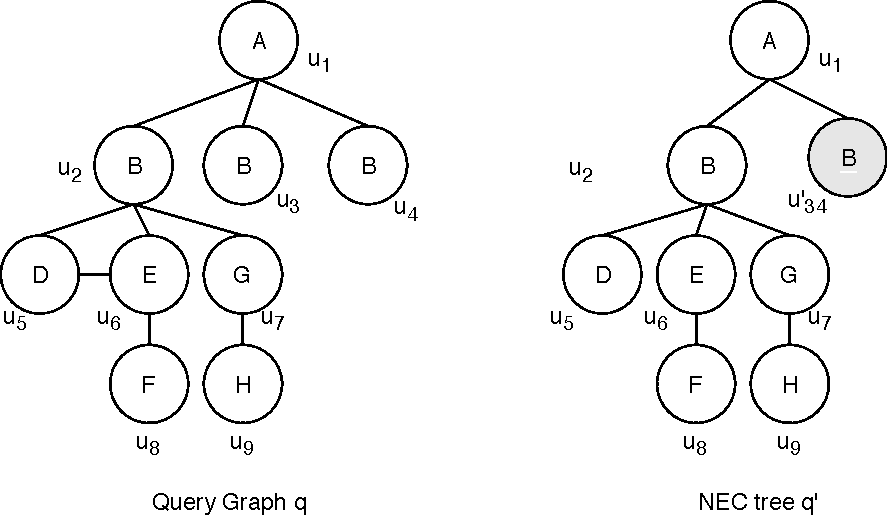
\includegraphics[width=\textwidth]{images/nec.pdf} 
\caption[Query graph and NEC Tree]{A query graph and its corresponding NEC Tree} % The text in the square bracket is the caption for the list of figures while the text in the curly brackets is the figure caption
\label{fig:gallery} 
\end{figure}


This algorithm was proposed in \cite{turbo}. $Turbo_{ISO}$ uses the concept of Neighbourhood Equivalence Class (NEC). Two vertices are said to be in an NEC if:
\begin{enumerate}
    \item They have same labels.
    \item The have exactly same subtrees (considering undirected graphs).
\end{enumerate}
Figure 2.1 shows a query graph and it's equivalent NEC tree.
In figure 2, $u_2$ and $u_3$ follow the above 2 rules and hence belong to the same NEC ($u^{'}_{2,3}$).
Matching time can be reduced using this concept as number of vertices that are to be matched will be reduced. Using NEC tree, we can reduce the number of call by huge margin as calls for vertices that are identically matching will be made only once. However, in order to generate all the matches, we will have to permute all the combinations for every NEC.